% !TEX root = ../../main.tex

\section{Thermodynamics of adsorption}

As mentioned in the introduction \todo{reference}, adsorption 
is a consequence of intermolecular attraction between the 
material surface and the molecules of the fluid. The sum of 
all interactions accounts for the depth of the potential 
well and therefore for the energy corresponding to the 
process. As this energy is net positive adsorption is an
overall exothermic phenomenon.

However, in order to make the transition from a molecular 
viewpoint to a macroscale bulk fluid representation of 
adsorption, the thermodynamics of the process must be 
clearly defined.

\subsection{The Gibbs surface excess approach}

A description of the adsorbed phase can be made through the change
in density or concentration of the fluid starting from the 
adsorbent surface. When represented as such, the density 
has a maxima in the immediate zone close to the surface and then
decreases until attaining the density of the bulk fluid.
However, when defined as such the boundary between the 
adsorbed phase and the bulk phase is difficult to pinpoint.
In some cases, such as adsorption in porous materials, the 
adsorbed phase can be taken as total pore volume, but in 
most cases it is useful to refer to the Gibbs surface 
excess approach of quantifying the amount adsorbed.

This concept describes the adsorbed phase only in terms
of an \textit{excess} from the properties of the bulk phase. 
As long as the volume of the adsorbed layer can be considered 
negligible and the concentration of adsorbate in the bulk 
phase is low, the total amount adsorbed and the surface excess
amount may be considered equal.

\subsection{Enthalpy of adsorption}

\begin{figure}[htb]
    \centering

    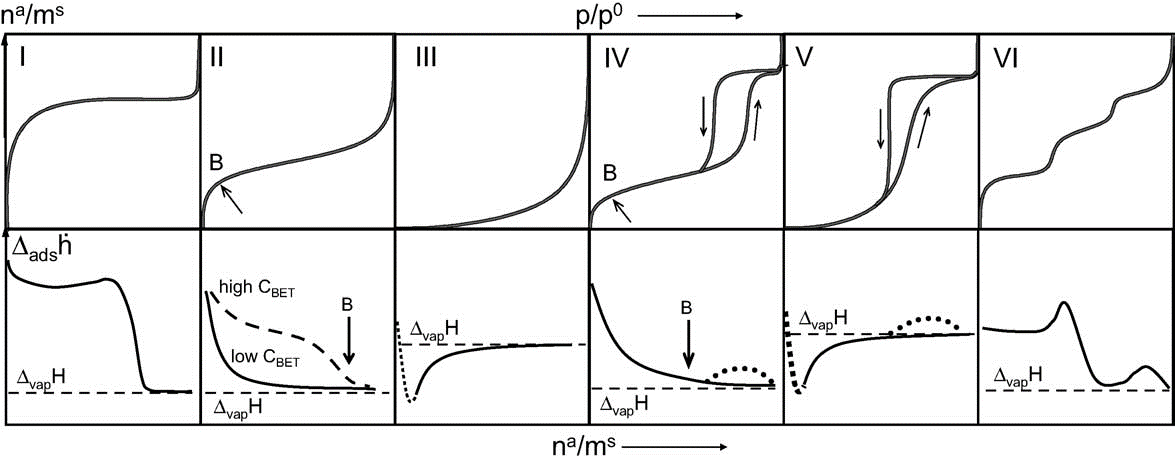
\includegraphics[width=\linewidth]{enthalpy-curves}
    \caption{
      General enthalpy curves corresponding to different 
      IUPAC-defined isotherm 
      types\cite{llewellynGasAdsorptionMicrocalorimetry2005}.
    }%
    \label{calo:fig:enthalpy-iupac-iso}

\end{figure}


\subsection{}